\section{Simulation Results}

In this section, we will provide the simulation results of the non-ideal Flyback Converter circuit for two different source (input) voltage level.

In the simulations, we will use the open loop model of the Flyback Converter circuit. Therefore, the duty cycle of the converter switch will be controlled by hand (using a PWM Generator block in Simulink).

The simulations will be much more detailed compared to the simulations provided in the Simulation Report, where we used the ideal Flyback Converter circuit model with the non-idealities of the circuit components and elements are ignored. However, in this report, we will make our similations including the non-idealities of the converter circuit components and elements. The non-ideal semiconductor characteristics for the MOSFET switch and the diode will be included to the simulations. We will also include the non-idealities of the output capacitor. Furthermore, the non-idealities in the magnetic design such as the coil resistances of the primary and the secondary side windings of the transformer and the leakage inductances of the primary and the secondary side windings of the transformer will be included in the simulations.

The non-idealities of the converter circuit components will be taken from their data sheet, and inserted into the simulation model.

The non-idealities in the magnetic design of the transformer such as coil resistances and the leakage inductance will be taken from the analytical calculations provided in the magnetic design section.

The following Figure \ref{fig:fly_schema} shows the Simulink model of the non-ideal Flyback Converter circuit. 

\begin{figure}[H]
\begin{center}
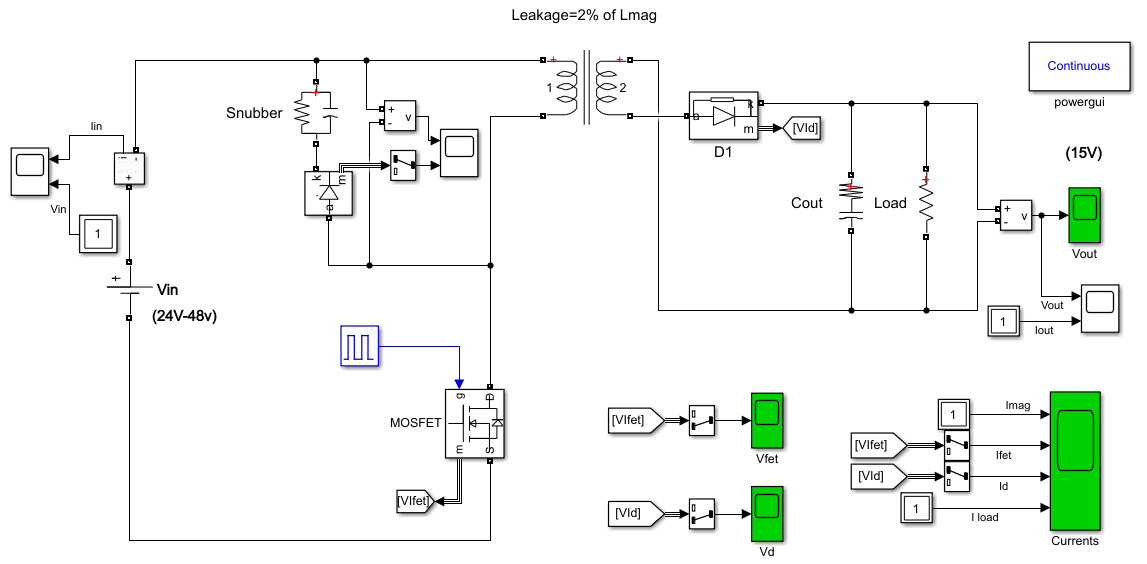
\includegraphics[width=1\textwidth]{figures/flyback_schematic.png}
\caption{Simulink Schematic of the Flyback Converter Circuit}
\label{fig:fly_schema}
\end{center}
\end{figure}

If we investigate this simulation model from its input to output about what is included and what is not included, we will, first of all, notice that we have included an RCD snubber to the primary side of the transformer. This RCD snubber is included in the simulation model due to the transformer leakage inductances. The close view of the used RCD snubber is shown in Figure \ref{fig:fly_snubber}, below.

\begin{figure}[H]
\begin{center}
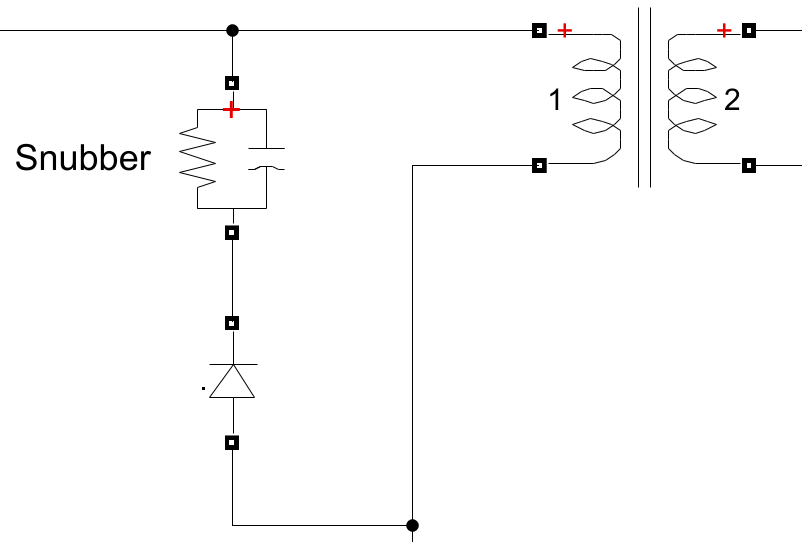
\includegraphics[width=0.4\textwidth]{simulations/snubber.png}
\caption{RCD Snubber Circuit}
\label{fig:fly_snubber}
\end{center}
\end{figure}

The primary side leakage inductance of the transformer increases the voltage stress on the MOSFET switch to infinity, which inevitably causes the MOSFET switch of the Flyback Converter to blow up, and hence resulting in circuit failures.

In order to prevent the voltage spikes that goes to infinity and to reduce the voltage stress over the MOSFET switch of the converter, we included an RCD snubber across the primary terminals of the transformer. The designed RCD snubber circuit provides the leakage inductance current a path to discharge over itself and the parallel RC circuit of the snubber. As a result, we provide a safe path for the leakage inductance current to flow, which reduces the voltage and current stresses over the MOSFET switch of the converter during its off (open) period.

The resistance R and the capacitance C parameters of the designed RCD snubber is as given below.

$$ R_S = 10\;k\ohm $$
$$ C_S = 47\;nF $$

Without the RCD snubber, the MOSFET voltage makes a spike and goes to infinity, which would undoubtedly damage the MOSFET and the break the converter circuit operation.

Next, as mentioned, we have also included the coil resistances and the leakage inductances of the primary and the secondary windings of the designed transformer in the simulation.

The following Figure \ref{fig:trans_para} shows the parameters entered to the linear transformer block in the simulation model.

\begin{figure}[H]
\begin{center}
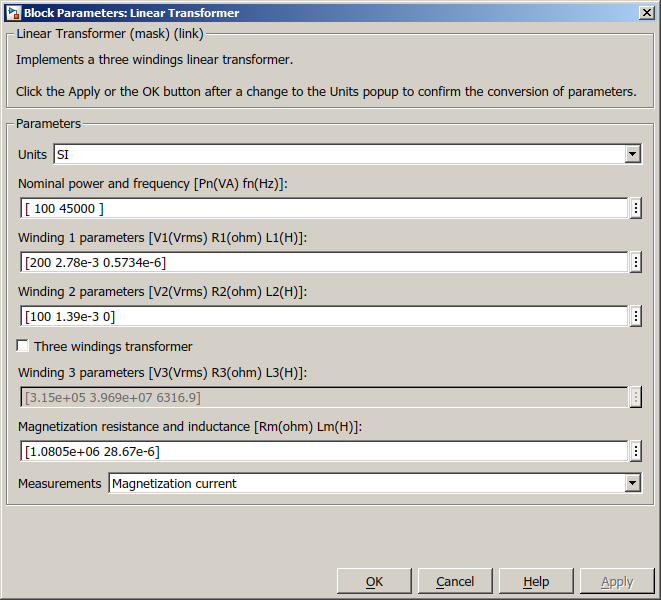
\includegraphics[width=0.4\textwidth]{simulations/transformer_para.png}
\caption{Transformer Block Parameters}
\label{fig:trans_para}
\end{center}
\end{figure}

We have entered the calculated coil resistances of the primary and the secondary windings of the designed transformer as calculated in the magnetic design section.

The entered coil resistance values are as follows:

$$ R_{pri,ac} = 2.78\;m\ohm $$
$$ R_{sec,ac} = 1.39\;m\ohm $$

We also entered the total leakage inductance of the primary and the secondary windings of the transformer as the 2\% of the magnetizing inductance of the transformer.

$$ L_m = 28.67\;\micro H $$

$$ L_{leakage} = 0.02\times L_m $$
$$ L_{leakage} = 0.02\times 28.67 = 0.5734\;\micro H $$

The total leakage inductance of the primary and the secondary windings of the transformer is included in the primary side of the transformer as shown in Figure \ref{fig:trans_para}.

Next, we have also included the non-idealities of the selected output capacitor. We included the ESR value of the selected capacitor to the simulation model.

The ESR value of the output filter capacitor is given as follows.

$$ R_{ESR} = 20\;m\ohm $$

Finally, we have also included the non-idealities of the semiconductor devices: MOSFET and diode. The non-idealities like on resistance and forward voltage drop are taken from their datasheet, and included in the simulation model.

The following figures show the included parameters for the semiconductor devices: MOSFET and diode.

\begin{figure}[H]
\begin{center}
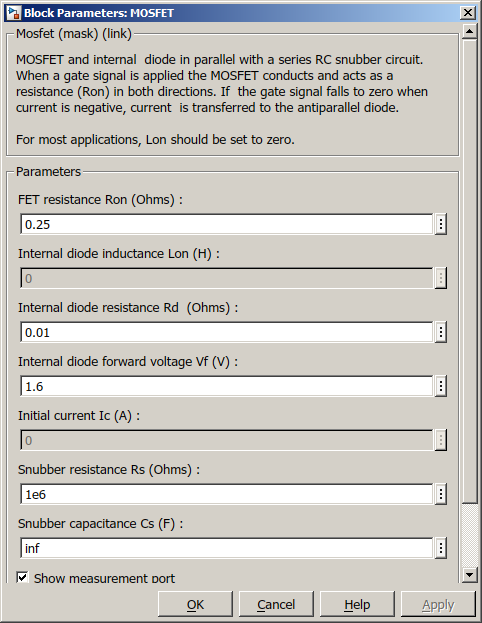
\includegraphics[width=0.4\textwidth]{simulations/mosfet_para.png}
\caption{MOSFET Block Parameters}
\label{fig:mosfet_para}
\end{center}
\end{figure}

\begin{figure}[H]
\begin{center}
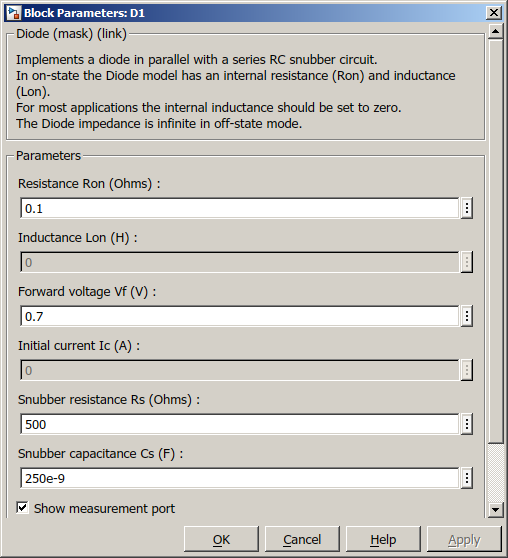
\includegraphics[width=0.4\textwidth]{simulations/diode_para.png}
\caption{Diode Block Parameters}
\label{fig:diode_para}
\end{center}
\end{figure}

Hence, we have completed the explanation of the included non-idealities in the simulation model. 

Now, we will explore the simulation results of the constructed non-ideal Flyback Converter circuit model for different source (input) voltage values.

\subsection{Simulation Results for $V_{in} = 24V$}

In this subsection, the simulation results of the constructed non-ideal Flyback Converter are presented for the source (input) voltage of 24V.

We have obtained the duty cycle value D which makes the average output voltage equal to 15V at steady-state as 60.4\% after a number of trials. This duty cycle value was determined as 52.7\% for the ideal Flyback Converter circuit model in the Simulation Report. However, in this case, it is required to increase this duty cycle value to 60.4\% due to the additional voltage drop effects of the non-idealities in the circuit components.

$$ D = 60.4\% $$

The Figure \ref{fig:tran_out24} shows the transient waveform of the output voltage of the converter for the source voltage of 24V.

\begin{figure}[H]
\begin{center}
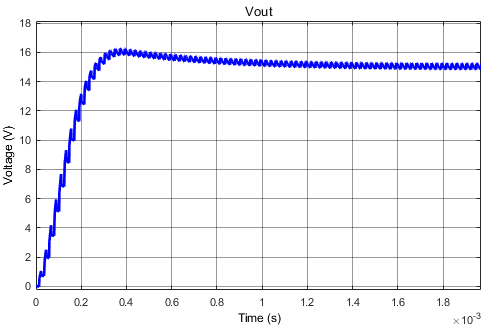
\includegraphics[width=0.7\textwidth]{figures/Vout_transient_24.png}
\caption{Transient Output Voltage Waveform of the Flyback Converter}
\label{fig:tran_out24}
\end{center}
\end{figure}

The steady-state waveform of the output voltage of the converter circuit for the source voltage of 24V is shown in Figure \ref{fig:out24}.

\begin{figure}[H]
\begin{center}
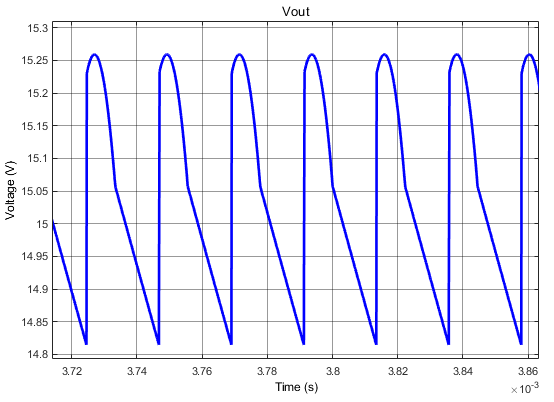
\includegraphics[width=0.7\textwidth]{figures/Vout_24.png}
\caption{Output Voltage Waveform of the Flyback Converter}
\label{fig:out24}
\end{center}
\end{figure}

It is observed that the output voltage oscillates around 15V on average. The peak value of the output voltage is measured as 15.26V, and the minimum value of the output voltage is measured as 14.81V. Hence, the steady-state peak to peak ripple at the output voltage of the converter is computed as 0.45V. This peak to peak ripple value is observed to be less than the maximum of 0.6V peak to peak ripple specified in the project limitations for the output voltage.

$$ \Delta V_{out} = 0.45V < 0.60V $$

The steady-state waveforms of the output voltage and the load current of the converter circuit for the source voltage of 24V are shown on the same plot in Figure \ref{fig:viout_24}.

\begin{figure}[H]
\begin{center}
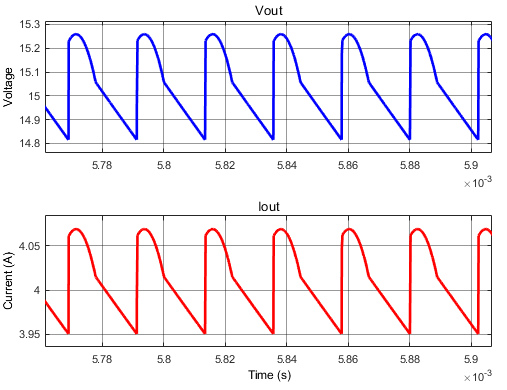
\includegraphics[width=0.7\textwidth]{figures/V_I_out_24.png}
\caption{Output Voltage and Load Current Waveforms of the Flyback Converter}
\label{fig:viout_24}
\end{center}
\end{figure}

It is observed from the load current waveform that it has an average of 4A, and oscillates around 4A. The maximum load current is equal to 4.07A while the minimum load current is equal to 3.95A. As a result, there is a 0.12A peak to peak ripple in the load current.

The steady-state current waveforms of magnetizing inductor, MOSFET switch and diode of the converter circuit for the source voltage of 24V are shown on the same plot in Figure \ref{fig:currents24}.

\begin{figure}[H]
\begin{center}
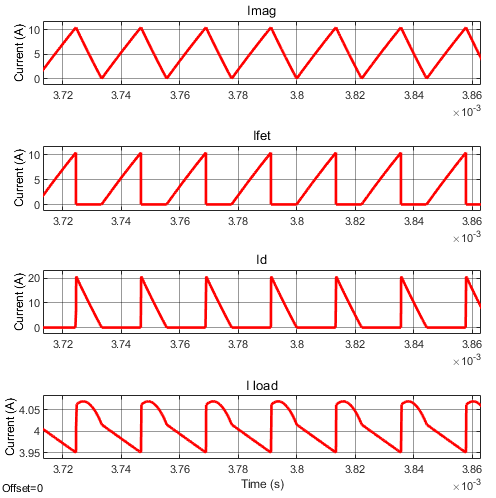
\includegraphics[width=0.7\textwidth]{figures/currents_24.png}
\caption{Current Waveforms of the Flyback Converter}
\label{fig:currents24}
\end{center}
\end{figure}

It is observed that the maximum repetitive current through the MOSFET switch is equal to 10A. In addition, the maximum repetitive current through the diode is approximately equal to 20A.

The peak repetitive current though the diode is the two times that of the MOSFET switch due to the 2:1 turns ratio between the transformer primary and secondary winding ($N_P/N_S = 2$). This makes the current levels at the secondary side of the transformer double of the current levels at the primary side of the transformer.

It is also observed that the magnetizing inductor current changes between 0A and 10A. It is also seen from the magnetizing inductor current that the converter circuit is operating slightly in the DCM mode. The magnetizing inductance current drops to 0A in each switching cycle.

Furthermore, we can state that the frequency of ripples in the output voltage, load current, MOSFET current and diode current is equal to the switching frequency $f_s$, which is equal to 45 kHz. As a result, the presented voltage and current waveforms has a ripple frequency of 45 kHz.

The MOSFET voltage waveform of the Flyback Converter circuit is shown in Figure \ref{fig:mos24}, below.

\begin{figure}[H]
\begin{center}
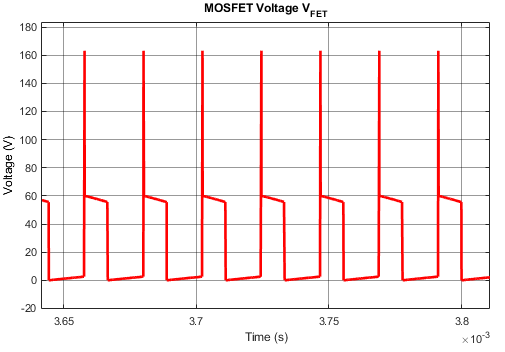
\includegraphics[width=0.7\textwidth]{figures/V_FET_24.png}
\caption{MOSFET Voltage Waveform of the Flyback Converter}
\label{fig:mos24}
\end{center}
\end{figure}

It is observed that maximum voltage stress over the MOSFET during its off (open) period is normally equal to around 60V. However, due to the leakage inductance of the transformer, we observe some voltage spikes in the MOSFET voltage waveform during the turn off operations of the switch. These voltage spikes are present despite the existence of the RCD snubber in the simulation model. However, the magnitude of the voltage spikes are greatly reduced and limited thanks to the existence of the RCD snubber on the primary side of the transformer. Normally, we would expect to see voltage spikes with a magnitude of around infinity on the MOSFET voltage in the absence of the RCD snubber. However, in the presence of the RCD snubber, we observe that the peak amplitude of the voltage spikes in the MOSFET voltage waveform is limited to around 160V as seen from Figure \ref{fig:mos24} above.

The selected commercial MOSFET model STP17NK40ZFP is able to withstand the drain to source voltages as high as 400V. This indicates that the selected switch model is able to withstand the measured voltage spike with a peak of 160V.

The diode voltage waveform of the Flyback Converter circuit is shown in Figure \ref{fig:diode24}, below.

\begin{figure}[H]
\begin{center}
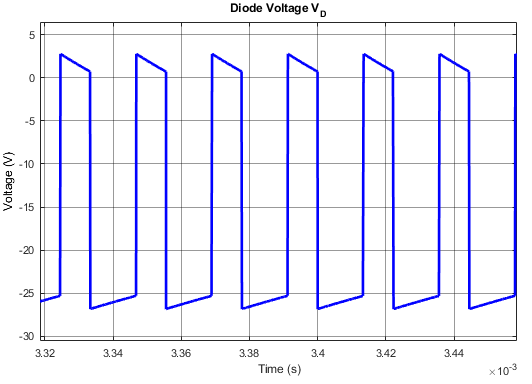
\includegraphics[width=0.7\textwidth]{figures/V_diode_24.png}
\caption{Diode Voltage Waveform of the Flyback Converter}
\label{fig:diode24}
\end{center}
\end{figure}

It is observed that the maximum reverse voltage across the diode is around -25V. The selected commercial diode model has a peak repetitive reverse blocking voltage rating of 100V. This result shows that the selected diode is able to operate properly under these steady-state conditions.

The snubber circuit voltage and current waveforms of the Flyback Converter circuit are shown in Figure \ref{fig:snubber24}, below.

\begin{figure}[H]
\begin{center}
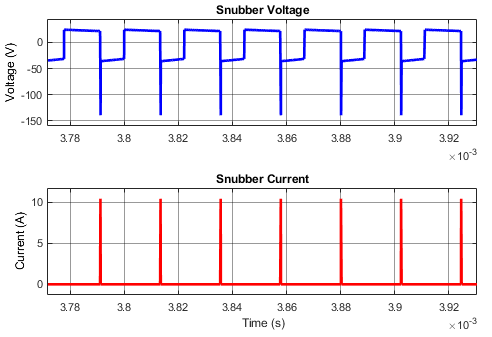
\includegraphics[width=0.7\textwidth]{figures/snubber_24.png}
\caption{RCD Snubber Voltage and Current Waveforms of the Flyback Converter}
\label{fig:snubber24}
\end{center}
\end{figure}

The input current waveform of the Flyback Converter circuit is shown in Figure \ref{fig:Iin24}, below.

\begin{figure}[H]
\begin{center}
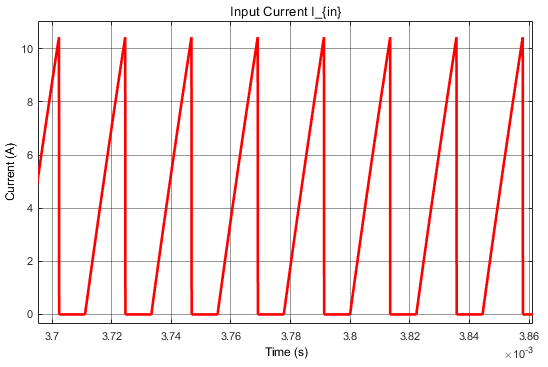
\includegraphics[width=0.7\textwidth]{figures/I_in_24.png}
\caption{Input Current Waveform of the Flyback Converter}
\label{fig:Iin24}
\end{center}
\end{figure}

The input current has a peak of approximately 11A in steady-state operation. The average input current is equal to 3.226A.

The Table \ref{tab:sim24} below shows the average voltage, current and power values obtained from the simulations of the Flyback Converter circuit with $V_{in} = 24V$. 

\begin{table}[H]
    \centering
    \caption{Average Voltage, Current and Power Values Obtained from Simulation}
    \begin{tabular}{|c|c|c|c|c|c|}
    \hline
\textbf{Parameter}   & \textbf{Value}          & \textbf{Parameter}      & \textbf{Value}          & \textbf{Parameter} & \textbf{Value}         \\ \hline
$V_{in}$ & 24V & $I_{in}$ & 3.226A & $P_{in}$ & 77.43W \\ \hline
$V_{out}$ & 15.04V & $I_{out}$ & 4.011A & $P_{out}$ & 60.34W \\ \hline
$I_D$ & 4.012A & $I_{FET}$ & 3.222A & $\eta$ & 78\% \\ \hline
$V_{out(max)}$ & 15.26V & $V_{out(min)}$ & 14.81V & $\Delta V_{out}$ & 0.45V \\ \hline
    \end{tabular}
    \label{tab:sim24}
\end{table}

Then, the efficiency of the Flyback Converter circuit for the input voltage $V_{in} = 24V$ is obtained as follows:

\begin{align}
    Efficiency = \eta = \frac{P_{out}}{P_{in}}
    \label{eqn:eff24}
\end{align}

$$ Efficiency = \eta = \frac{60.34W}{77.43W} = 0.78\;(78\%) $$

Hence, it is seen from the simulations of the non-ideal Flyback Converter circuit in Simulink that it has an efficiency of around 78\% for the source voltage of 24V. This efficiency level is satisfactory considering that all possible non-idealities in the converter circuit components are included in the simulation model except for the core losses of the designed transformer. 

The detailed efficiency analysis of the Flyback Converter circuit including the core losses of the designed transformer is presented in the Efficiency Analysis section of the report.

It is also observed from Table \ref{tab:sim24} that the output voltage ripple $\Delta V_{out}$ is equal to 0.45V, which is less than the project limitations of 0.6V (4\% of the output average voltage). This result shows that the designed Flyback Converter circuit is able to meet the project specifications defined on the output voltage limitations successfully.

$$ \Delta V_{out} = 0.45V < 0.60V $$

\subsection{Simulation Results for $V_{in} = 48V$}

In this subsection, the simulation results of the constructed non-ideal Flyback Converter are presented for the source (input) voltage of 48V.

We have obtained the duty cycle value D which makes the average output voltage equal to 15V at steady-state as 29.4\% after a number of trials. This duty cycle value was determined as 26.25\% for the ideal Flyback Converter circuit model in the Simulation Report. However, in this case, it is required to increase this duty cycle value to 29.4\% due to the additional voltage drop effects of the non-idealities in the circuit components.

$$ D = 29.4\% $$

The Figure \ref{fig:tran_out48} shows the transient waveform of the output voltage of the converter for the source voltage of 48V.

\begin{figure}[H]
\begin{center}
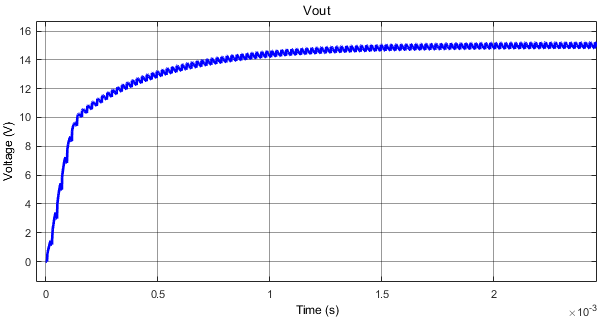
\includegraphics[width=0.7\textwidth]{figures/Vout_transient2_48.png}
\caption{Transient Output Voltage Waveform of the Flyback Converter}
\label{fig:tran_out48}
\end{center}
\end{figure}

The steady-state waveform of the output voltage of the converter circuit for the source voltage of 48V is shown in Figure \ref{fig:out48}.

\begin{figure}[H]
\begin{center}
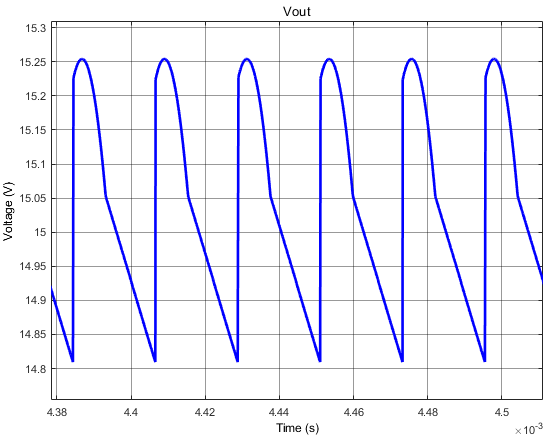
\includegraphics[width=0.7\textwidth]{figures/Vout_48.png}
\caption{Output Voltage Waveform of the Flyback Converter}
\label{fig:out48}
\end{center}
\end{figure}

It is observed that the output voltage oscillates around 15V on average. The peak value of the output voltage is measured as 15.25V, and the minimum value of the output voltage is measured as 14.81V. Hence, the steady-state peak to peak ripple at the output voltage of the converter is calculated as 0.44V. This peak to peak ripple value is observed to be less than the maximum of 0.6V peak to peak ripple specified in the project limitations for the output voltage.

$$ \Delta V_{out} = 0.44V < 0.60V $$

The steady-state waveforms of the output voltage and the load current of the converter circuit for the source voltage of 48V are shown on the same plot in Figure \ref{fig:viout_48}.

\begin{figure}[H]
\begin{center}
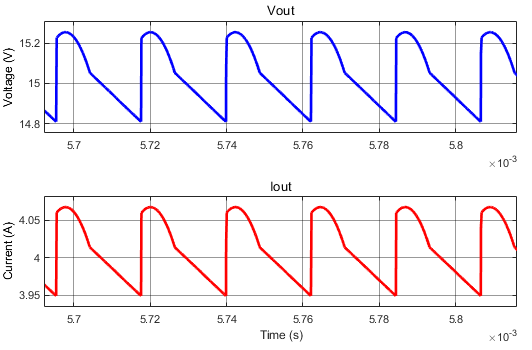
\includegraphics[width=0.7\textwidth]{figures/V_I_out_48.png}
\caption{Output Voltage and Load Current Waveforms of the Flyback Converter}
\label{fig:viout_48}
\end{center}
\end{figure}

It is observed from the load current waveform that it has an average of 4A, and oscillates around 4A. The maximum load current is equal to 4.07A while the minimum load current is equal to 3.95A. As a result, there is a 0.12A peak to peak ripple in the load current.

The steady-state current waveforms of magnetizing inductor, MOSFET switch and diode of the converter circuit for the source voltage of 48V are shown on the same plot in Figure \ref{fig:currents48}.

\begin{figure}[H]
\begin{center}
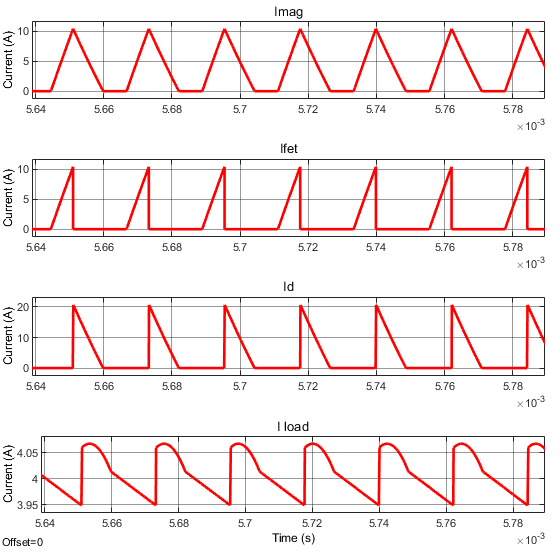
\includegraphics[width=0.7\textwidth]{figures/currents_48.png}
\caption{Current Waveforms of the Flyback Converter}
\label{fig:currents48}
\end{center}
\end{figure}

It is observed that the maximum repetitive current through the MOSFET switch is equal to 10A. In addition, the maximum repetitive current through the diode is approximately equal to 20A.

The peak repetitive current though the diode is the two times that of the MOSFET switch due to the 2:1 turns ratio between the transformer primary and secondary winding ($N_P/N_S = 2$). This makes the current levels at the secondary side of the transformer double of the current levels at the primary side of the transformer.

It is also observed that the magnetizing inductor current changes between 0A and 10A. We can also clearly observe the DCM mode of operation of the converter circuit for the source voltage value of 48V. The magnetizing inductance current drops down to 0A in each switching cycle, and stays at 0A for a short period until the next switching cycle begins.

Furthermore, we can state that the frequency of ripples in the output voltage, load current, MOSFET current and diode current is equal to the switching frequency $f_s$, which is equal to 45 kHz. As a result, the presented voltage and current waveforms has a ripple frequency of 45 kHz.

The MOSFET voltage waveform of the Flyback Converter circuit is shown in Figure \ref{fig:mos48}, below.

\begin{figure}[H]
\begin{center}
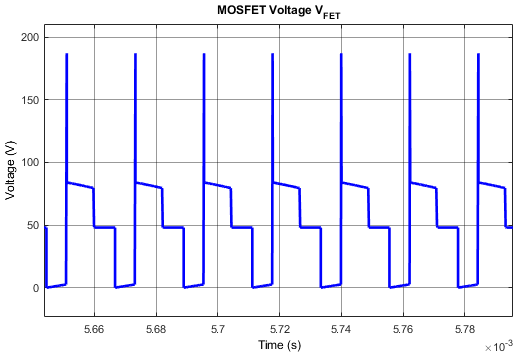
\includegraphics[width=0.7\textwidth]{figures/V_FET_48.png}
\caption{MOSFET Voltage Waveform of the Flyback Converter}
\label{fig:mos48}
\end{center}
\end{figure}

It is observed that maximum voltage stress over the MOSFET during its off (open) period is normally equal to around 80V. However, due to the leakage inductance of the transformer, we observe some voltage spikes in the MOSFET voltage waveform during the turn off operations of the switch. These voltage spikes are present despite the existence of the RCD snubber in the simulation model. However, the magnitude of the voltage spikes are greatly reduced and limited thanks to the existence of the RCD snubber on the primary side of the transformer. Normally, we would expect to see voltage spikes with a magnitude of around infinity on the MOSFET voltage in the absence of the RCD snubber. However, in the presence of the RCD snubber, we observe that the peak amplitude of the voltage spikes in the MOSFET voltage waveform is limited to around 200V as seen from Figure \ref{fig:mos48} above.

The selected commercial MOSFET model STP17NK40ZFP is able to withstand the drain to source voltages as high as 400V. This indicates that the selected switch model is able to withstand the measured voltage spike with a peak of 200V.

We are also able to observe the DCM operation of the converter circuit for the source voltage value of 48V from the MOSFET voltage waveform. It is seen that the MOSFET voltage drops down from approximately 80V to 48V during the off (open) period off the switch. This action occurs at the moment when the magnetizing inductor current becomes zero. When the magnetizing inductance current becomes zero, the voltage across the MOSFET switch terminals is equal to the source voltage, which is 48V. Therefore, the MOSFET voltage drops down from 80V to 48V in the middle of the off (open) period of the switch when the magnetizing inductor current becomes zero.

The diode voltage waveform of the Flyback Converter circuit is shown in Figure \ref{fig:diode48}, below.

\begin{figure}[H]
\begin{center}
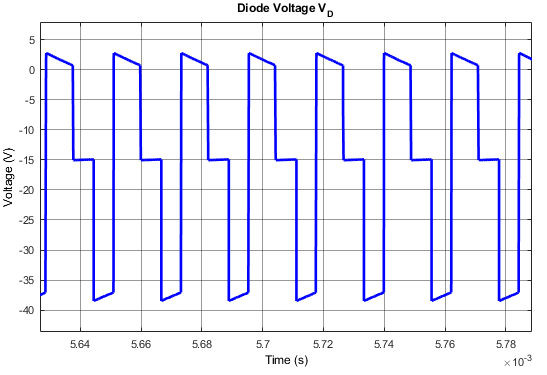
\includegraphics[width=0.7\textwidth]{figures/V_D_48.png}
\caption{Diode Voltage Waveform of the Flyback Converter}
\label{fig:diode48}
\end{center}
\end{figure}

It is observed that the maximum reverse voltage across the diode is around -40V. The selected commercial diode model has a peak repetitive reverse blocking voltage rating of 100V. This result shows that the selected diode is able to operate properly under these steady-state conditions.

During the on (closed) period of the MOSFET switch of the Flyback Converter, the diode is off, and hence not conducting. The reverse voltage over the diode is equal to the negative sum of the output voltage $V_o$ and the secondary side terminal voltage of the transformer $V_2$. During the on (closed) period of the MOSFET switch, the primary side voltage of the transformer, $V_1$, is equal to the source voltage, which is 48V. Then, the secondary side voltage of the transformer during that period is equal to 24V since the transformer has a turns ratio of 2:1 from its primary to secondary ($N_P/N_S = 2$).

$$ V_1 = 48V $$

$$ V_2 = V_1\frac{N_S}{N_P} = 48\times\frac{5}{10} = 24V $$

Then, the reverse voltage over the diode is computed as -39V during that period.

$$ V_{diode} = - V_2 - V_{out} = -24-15 = -39V $$

When the MOSFET switch turns off, the stored magnetic energy in the magnetizing inductor is transferred to the secondary side (load side) of the transformer. Hence, the diode is on until the magnetizing inductance current drops down to 0A. Therefore, the diode voltage is equal to the forward voltage drop of the selected diode, which is equal to 0.7V, during that period. When the magnetizing inductance current becomes zero, the primary side terminals of the transformer is like short circuited with zero voltage. Hence, the secondary side terminals of the transformer is also short circuited. As a result, the diode turns off, and gets out of conduction when the magnetizing inductor current becomes zero. This means that the reverse voltage across the diode is equal to the negative of the output voltage, which is -15V. Therefore, the reverse voltage across the diode becomes -15V after the magnetizing inductance current becomes zero. The reverse diode voltage stays at -15V until the next switching cycle begins with the MOSFET switch turning on (closed) again. When the MOSFET switch is turned on (closed), the reverse voltage across the diode becomes -39V, again as explained above. This operation repeats itself in every switching period.

In short, we observe that the reverse diode voltage is equal to the negative of the output voltage, which is -15, during the time periods when the magnetizing inductance current is equal to zero (0A). This result also shows that the Flyback Converter circuit is operating in DCM mode for the source voltage of 48V.

The snubber circuit voltage and current waveforms of the Flyback Converter circuit are shown in Figure \ref{fig:snubber48}, below.

\begin{figure}[H]
\begin{center}
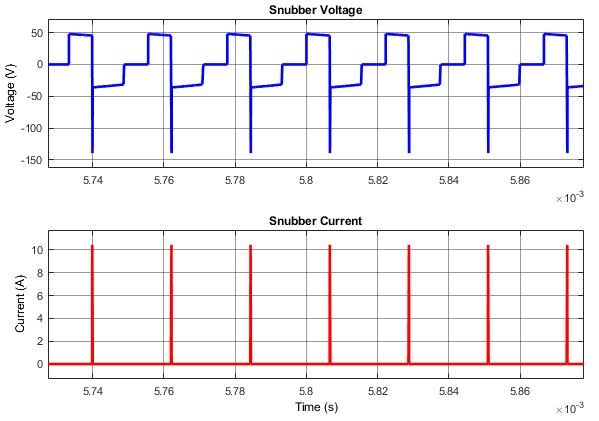
\includegraphics[width=0.7\textwidth]{figures/snubber_48.png}
\caption{RCD Snubber Voltage and Current Waveforms of the Flyback Converter}
\label{fig:snubber48}
\end{center}
\end{figure}

The input current waveform of the Flyback Converter circuit is shown in Figure \ref{fig:Iin48}, below.

\begin{figure}[H]
\begin{center}
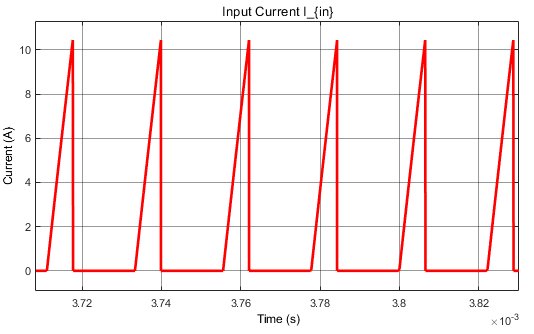
\includegraphics[width=0.7\textwidth]{figures/Iin_48.png}
\caption{Input Current Waveform of the Flyback Converter}
\label{fig:Iin48}
\end{center}
\end{figure}

The input current has a peak of approximately 11A in steady-state operation. The average input current is equal to 1.553A.

The Table \ref{tab:sim48} below shows the average voltage, current and power values obtained from the simulations of the Flyback Converter circuit with $V_{in} = 48V$. 

\begin{table}[H]
    \centering
    \caption{Average Voltage, Current and Power Values Obtained from Simulation}
    \begin{tabular}{|c|c|c|c|c|c|}
    \hline
\textbf{Paremeter}   & \textbf{Value}          & \textbf{Parameter}      & \textbf{Value}          & \textbf{Parameter} & \textbf{Value}         \\ \hline
$V_{in}$ & 48V & $I_{in}$ & 1.553A & $P_{in}$ & 74.56W \\ \hline
$V_{out}$ & 15.04V & $I_{out}$ & 4.01A & $P_{out}$ & 60.31W \\ \hline
$I_D$ & 4.011A & $I_{FET}$ & 1.549A & $\eta$ & 81\% \\ \hline
$V_{out(max)}$ & 15.25V & $V_{out(min)}$ & 14.81V & $\Delta V_{out}$ & 0.44V \\ \hline
    \end{tabular}
    \label{tab:sim48}
\end{table}

Then, the efficiency of the Flyback Converter circuit for the input voltage $V_{in} = 48V$ is obtained as follows:

\begin{align}
    Efficiency = \eta = \frac{P_{out}}{P_{in}}
    \label{eqn:eff48}
\end{align}

$$ Efficiency = \eta = \frac{60.31W}{74.56W} = 0.81\;(81\%) $$

Hence, it is seen from the simulations of the non-ideal Flyback Converter circuit in Simulink that it has an efficiency of around 81\% for the source voltage of 48V. This efficiency level is satisfactory considering that all possible non-idealities in the converter circuit components are included in the simulation model except for the core losses of the designed transformer. 

The detailed efficiency analysis of the Flyback Converter circuit including the core losses of the designed transformer is presented in the Efficiency Analysis section of the report.

It is also observed from Table \ref{tab:sim48} that the output voltage ripple $\Delta V_{out}$ is equal to 0.44V, which is less than the project limitations of 0.6V (4\% of the output average voltage). This result shows that the designed Flyback Converter circuit is able to meet the project specifications  defined on the output voltage limitations successfully.

$$ \Delta V_{out} = 0.44V < 0.60V $$